%
% $RCSfile: review.tex,v $
%
% Copyright (C) 2002-2008. Christian Heller.
%
% Permission is granted to copy, distribute and/or modify this document
% under the terms of the GNU Free Documentation License, Version 1.1 or
% any later version published by the Free Software Foundation; with no
% Invariant Sections, with no Front-Cover Texts and with no Back-Cover
% Texts. A copy of the license is included in the section entitled
% "GNU Free Documentation License".
%
% http://www.cybop.net
% - Cybernetics Oriented Programming -
%
% http://www.resmedicinae.org
% - Information in Medicine -
%
% Version: $Revision: 1.1 $ $Date: 2008-08-19 20:41:08 $ $Author: christian $
% Authors: Christian Heller <christian.heller@tuxtax.de>
%

\chapter{Review}
\label{review_heading}

\begin{flushright}
    \textsl{
        Knowledge can create problems.\\
        It is not through ignorance that we can solve them.
    }\\
    \textsc{Isaac Asimov}
\end{flushright}

This chapter will review the whole work in brief. It begins with firstly,
\emph{validating} the achieved results in comparison to the aims set initially.
Secondly, a short discussion will \emph{evaluate} these results once more,
before a third section mentions \emph{limits} of the proposed solution.

%
% $RCSfile: validation.tex,v $
%
% Copyright (C) 2002-2008. Christian Heller.
%
% Permission is granted to copy, distribute and/or modify this document
% under the terms of the GNU Free Documentation License, Version 1.1 or
% any later version published by the Free Software Foundation; with no
% Invariant Sections, with no Front-Cover Texts and with no Back-Cover
% Texts. A copy of the license is included in the section entitled
% "GNU Free Documentation License".
%
% http://www.cybop.net
% - Cybernetics Oriented Programming -
%
% http://www.resmedicinae.org
% - Information in Medicine -
%
% Version: $Revision: 1.1 $ $Date: 2008-08-19 20:41:09 $ $Author: christian $
% Authors: Christian Heller <christian.heller@tuxtax.de>
%

\section{Validation}
\label{validation_heading}
\index{CYBOP Validation}

The state-of-the-art chapters \ref{software_engineering_process_heading},
\ref{physical_architecture_heading} and \ref{logical_architecture_heading}, at
the beginning of this work, dealt with the \emph{Software Engineering Process}
(SEP), the \emph{Physical-} and \emph{Logical Architecture} of information
systems. A rather large number of existing software design concepts were
investigated, and some of their aspects criticised, before chapter
\ref{extended_motivation_heading} suggested a new approach for their
improvement. Many of its new concepts and ideas stem from nature or other
disciplines of science, which is why that programming approach was given the
attribute \emph{cybernetics-oriented} (CYBOP). Part \ref{contribution_heading}
then proposed a slightly different view on how to abstract knowledge in form of
software, which part \ref{proof_heading} tried to prove by introducing a
language and interpreter, as well as an application prototype using both.

In order to validate the results of this work, the following sub sections
explain once again in short why many of the problems identified in today's
programming language concepts are solved when applying CYBOP principles.

%
% $RCSfile: distinction_of_statics_and_dynamics.tex,v $
%
% Copyright (C) 2002-2008. Christian Heller.
%
% Permission is granted to copy, distribute and/or modify this document
% under the terms of the GNU Free Documentation License, Version 1.1 or
% any later version published by the Free Software Foundation; with no
% Invariant Sections, with no Front-Cover Texts and with no Back-Cover
% Texts. A copy of the license is included in the section entitled
% "GNU Free Documentation License".
%
% http://www.cybop.net
% - Cybernetics Oriented Programming -
%
% http://www.resmedicinae.org
% - Information in Medicine -
%
% Version: $Revision: 1.1 $ $Date: 2008-08-19 20:41:06 $ $Author: christian $
% Authors: Christian Heller <christian.heller@tuxtax.de>
%

\subsection{Distinction of Statics and Dynamics}
\label{distinction_of_statics_and_dynamics_heading}
\index{CYBOP Distinction of Statics and Dynamics}

A first major mistake in current language concepts and design solutions is the
mix-up of static and dynamic parts of software, that is pure application-domain
knowledge and its processing, close to hardware. It is the reason for:

\begin{itemize}
    \item[a] Abstraction gap between designed system architecture and implemented
        source code, in a SEP (section \ref{abstraction_gaps_heading})
    \item[b] Global data access via static class methods being insecure
        (section \ref{global_access_heading})
    \item[c] Bidirectional dependencies caused by some software patterns
        (section \ref{bidirectional_dependency_heading})
    \item[d] Usage of reflective techniques which are based on bidirectional
        dependencies and often cause broken type systems with circular
        references between super- and sub platform (section \ref{reflection_heading})
    \item[e] Spread functionality through crosscutting concerns and complicated
        handling of aspects (section \ref{aspect_oriented_programming_heading})
    \item[f] Memory leaks
    \item[g] Repeated implementation of the same platform-dependent functionality
    \item[h] Repeated usage and copying of the same software patterns (section
        \ref{pattern_systematics_heading})
\end{itemize}

Chapter \ref{statics_and_dynamics_heading} therefore recommended a strict distinction
of high-level static knowledge and low-level dynamic system control functionality.
The CYBOL language (chapter \ref{cybernetics_oriented_language_heading}) was
defined to express and specify knowledge in the most general sense; the CYBOI
interpreter (chapter \ref{cybernetics_oriented_interpreter_heading}) was
created to control a system based on CYBOL input.

\paragraph{a}

Since CYBOL knowledge templates are a complete formal description of an
application's architecture, they represent its implementation at the same time.
But that also means that the transfer of a system's design into a programming
language, as known from classical application development, becomes superfluous.
The \emph{Design-} and \emph{Implementation} phases are merged, so that a gap
does not exist anymore.

\paragraph{b}

Since CYBOI holds all knowledge in one single instance tree whose nodes can
be accessed along well-defined paths, data are not globally accessible anymore.

\paragraph{c}

Since parts of a knowledge model are accessed unidirectionally, bidirectional
dependencies are not an issue any longer.

\paragraph{d}

Since CYBOI is based on one standardised knowledge schema providing a
well-defined type structure which does not have to be changed at runtime, there
is neither a need nor a possibility for workarounds like reflective mechanisms
causing a broken type system. Because the knowledge schema's whole-part
hierarchy already provides meta information such as a part model's name and
kind of abstraction (comparable to an attribute's name and type hold by the
meta class of a class), one main reason for using reflective techniques like
meta classes thereby falls apart. A second reason that does not count any
longer is the provision of basic features (like persistence or communication)
through meta techniques; CYBOI already contains these features and may act as
universal communicator.

\paragraph{e}

Since CYBOI does provide all necessary low-level mechanisms, crosscutting
concerns become superfluous. These concerns usually want to achieve the same as
reflection in that they provide basic functionality to all parts of a system.
However, since CYBOL knowledge templates are free from low-level system control
information and contain pure domain knowledge instead, crosscutting concerns
and aspects are not a topic of interest any longer.

\paragraph{f}

Since CYBOI concentrates all knowledge models (instances) in one place, as
branches of one single knowledge tree, forgotten models can get smoothly
destroyed at application shutdown. Traditionally, special mechanisms like
\emph{Garbage Collectors} (GC) had to be applied to achieve this, because
systems written in classical languages leave it up to the programmer to
properly reference all instances. If a reference to one instance was lost, it
could not get destroyed and resided as leak in memory. Often, more and more
memory space got blocked that way, until all RAM space was taken and a computer
hung (crashed). In CYBOI, a reference to any instance is always available, via
the root of the knowledge tree.

\paragraph{g}

Since CYBOI contains all hardware-dependent functionality, the application
knowledge encoded in CYBOL templates or serialised models is truly
platform-neutral, easily switchable and exchangeable among systems. The
low-level system gets uninteresting; high-level knowledge is what application
developers can now concentrate on. Finally, the old dream of having knowledge
engineers (domain experts) working independently from software system engineers
might possibly be coming true.

\paragraph{h}

Since CYBOI already implements all necessary patterns, application developers
and domain experts are freed from the burden to learn and apply the same
software patterns again and again; they can now develop application systems
considering just one concept: that of hierarchical \emph{Composition}.

%
% $RCSfile: usage_of_a_double_hierarchy_knowledge_schema.tex,v $
%
% Copyright (C) 2002-2008. Christian Heller.
%
% Permission is granted to copy, distribute and/or modify this document
% under the terms of the GNU Free Documentation License, Version 1.1 or
% any later version published by the Free Software Foundation; with no
% Invariant Sections, with no Front-Cover Texts and with no Back-Cover
% Texts. A copy of the license is included in the section entitled
% "GNU Free Documentation License".
%
% http://www.cybop.net
% - Cybernetics Oriented Programming -
%
% http://www.resmedicinae.org
% - Information in Medicine -
%
% Version: $Revision: 1.1 $ $Date: 2008-08-19 20:41:09 $ $Author: christian $
% Authors: Christian Heller <christian.heller@tuxtax.de>
%

\subsection{Usage of a Double-Hierarchy Knowledge Schema}
\label{usage_of_a_double_hierarchy_knowledge_schema_heading}
\index{CYBOP Usage of a Double-Hierarchy Knowledge Schema}

A further problem that was identified in this work is the missing concept of
hierarchy, which is not inherent in types of the corresponding languages.
Moreover, knowledge structures are mixed up with meta information leading to:

\begin{itemize}
    \item[a] Inflexible static typing in system programming languages (section
        \ref{system_programming_heading})
    \item[b] Fragile base class problem when using inheritance (section
        \ref{fragile_base_class_heading})
    \item[c] Overly large source code due to encapsulation without sense
        (section \ref{encapsulation_heading})
    \item[d] Unpredictable behaviour and falsified contents due to container
        inheritance (section \ref{falsifying_polymorphism_heading})
    \item[e] Redundant code caused by concerns and difficult application of an
        ontological structure (section \ref{spread_functionality_heading})
    \item[f] Complicated, partly impossible serialisation of knowledge models
\end{itemize}

Chapter \ref{knowledge_schema_heading} therefore proposed a new knowledge
schema which considers structural- as well as meta information, in two
different hierarchies.

\paragraph{a}

Since type information is not fixed statically, it gets dynamically
configurable at runtime, leading to highly flexible application systems. There
is only one static data structure -- the standardised knowledge schema. It
holds meta information about the kind of abstraction (type) of the data
contained in it.

\paragraph{b}

Since runtime knowledge models in CYBOI rely on composition only, the fragile
base class problem caused by runtime type inheritance in object-oriented systems
does not occur.

\paragraph{c}

Since the CYBOI-internal knowledge structure is a container by default, it
also provides all necessary access procedures. Thousands of useless access
methods as known from object-oriented programming are avoided. The partial
security they provided can be replaced with other mechanisms. Since all
knowledge resides in just one instance tree, it is easy to apply any kind of
security checks, whenever a part of the knowledge tree gets accessed.

\paragraph{d}

Since each CYBOP knowledge template or -model is constructed as hierarchy, so
that containers of any kind can be emulated, problematic container inheritance
belongs to the past.

\paragraph{e}

Since CYBOP knowledge models are purely hierarchical, it gets easier to apply
ontological structures which bundle functionality, instead of spreading it in a
concern-like manner.

\paragraph{f}

Since all knowledge is modelled hierarchically, it is easily serialisable and
hence exchangeable.

%
% $RCSfile: separation_of_state_and_logic_knowledge.tex,v $
%
% Copyright (C) 2002-2008. Christian Heller.
%
% Permission is granted to copy, distribute and/or modify this document
% under the terms of the GNU Free Documentation License, Version 1.1 or
% any later version published by the Free Software Foundation; with no
% Invariant Sections, with no Front-Cover Texts and with no Back-Cover
% Texts. A copy of the license is included in the section entitled
% "GNU Free Documentation License".
%
% http://www.cybop.net
% - Cybernetics Oriented Programming -
%
% http://www.resmedicinae.org
% - Information in Medicine -
%
% Version: $Revision: 1.1 $ $Date: 2008-08-19 20:41:08 $ $Author: christian $
% Authors: Christian Heller <christian.heller@tuxtax.de>
%

\subsection{Separation of State- and Logic Knowledge}
\label{separation_of_state_and_logic_knowledge_heading}
\index{CYBOP Separation of State- and Logic Knowledge}

A third aspect causing troubles in software system design is the bundling of
state- and logic knowledge, known from object-oriented programming. It results
in:

\begin{itemize}
    \item[a] Difficult handling and repeated implementation of the same
        communication mechanisms (section \ref{misleading_tiers_heading})
    \item[b] Differing patterns complicating the handling of communication
        (section \ref{pattern_heading})
    \item[c] Bidirectional dependencies (circular references) between classes/
        objects in object-oriented systems, due to attribute-method bundling
        (section \ref{bidirectional_dependency_heading})
    \item[d] Pre-defined logic concepts in structured/ procedural- as well as
        object-oriented programming
\end{itemize}

Chapter \ref{state_and_logic_heading} therefore suggested a separation of
state- and logic concepts, in order to eliminate unnecessary inter-dependencies
and to be able to apply a unified translator architecture.

\paragraph{a}

Since low-level communication mechanisms are implemented in CYBOI,
application developers writing CYBOL knowledge templates do not have to bother
with these anymore.

\paragraph{b}

Since standard communication patterns are unified, the handling of
communication is simplified. Thanks to this unification, an extensible
translator architecture can be applied. Using it, any kind of abstract
knowledge model can be translated into any other. Universal communication
becomes possible.

\paragraph{c}

Since state- are split from logic concepts, many (partly bidirectional)
dependencies between knowledge models disappear, which reduces the coupling
between- and increases cohesion within models. Both kinds use exclusively
unidirectional relations. Additionally, logic- may access state models and each
other, but always unidirectionally.

\paragraph{d}

Since logic concepts (algorithms, workflows) are themselves modelled as CYBOL
knowledge templates, they become configurable. Traditionally, only structures
representing states are manipulatable at runtime; procedures representing logic
are fixed and cannot be altered.


%
% $RCSfile: evaluation.tex,v $
%
% Copyright (C) 2002-2008. Christian Heller.
%
% Permission is granted to copy, distribute and/or modify this document
% under the terms of the GNU Free Documentation License, Version 1.1 or
% any later version published by the Free Software Foundation; with no
% Invariant Sections, with no Front-Cover Texts and with no Back-Cover
% Texts. A copy of the license is included in the section entitled
% "GNU Free Documentation License".
%
% http://www.cybop.net
% - Cybernetics Oriented Programming -
%
% http://www.resmedicinae.org
% - Information in Medicine -
%
% Version: $Revision: 1.1 $ $Date: 2008-08-19 20:41:06 $ $Author: christian $
% Authors: Christian Heller <christian.heller@tuxtax.de>
%

\section{Evaluation}
\label{evaluation_heading}
\index{CYBOP Evaluation}

Having validated the results of this work, their impact on software design and
-engineering can be discussed and evaluated.

%
% $RCSfile: knowledge_triumvirate.tex,v $
%
% Copyright (C) 2002-2008. Christian Heller.
%
% Permission is granted to copy, distribute and/or modify this document
% under the terms of the GNU Free Documentation License, Version 1.1 or
% any later version published by the Free Software Foundation; with no
% Invariant Sections, with no Front-Cover Texts and with no Back-Cover
% Texts. A copy of the license is included in the section entitled
% "GNU Free Documentation License".
%
% http://www.cybop.net
% - Cybernetics Oriented Programming -
%
% http://www.resmedicinae.org
% - Information in Medicine -
%
% Version: $Revision: 1.1 $ $Date: 2008-08-19 20:41:07 $ $Author: christian $
% Authors: Christian Heller <christian.heller@tuxtax.de>
%

\subsection{Knowledge Triumvirate}
\label{knowledge_triumvirate_heading}
\index{CYBOP Knowledge Triumvirate}
\index{Knowledge Triumvirate}
\index{Schema}
\index{Template}
\index{Model}
\index{CYBOP}
\index{CYBOL}
\index{CYBOI}
\index{Fourth Generation Languages}
\index{4GL}
\index{Object Oriented Programming Systems}
\index{OOPS}
\index{Computer Aided Software Engineering}
\index{CASE}
\index{Functional Programming}
\index{Procedural Language}
\index{Structured- and Procedural Programming}
\index{SPP}
\index{Side Effect}
\index{Knowledge Tree}
\index{State and Logic}
\index{Object Oriented Programming}
\index{OOP}
\index{Tree Structure}

Chapter \ref{knowledge_schema_heading} introduced a new \emph{Schema} for
knowledge representation; chapter \ref{cybernetics_oriented_language_heading}
defined a language for knowledge specification, in form of \emph{Templates};
chapter \ref{cybernetics_oriented_interpreter_heading} described a system for
knowledge processing, that uses \emph{Models}.

\begin{figure}[ht]
    \begin{center}
        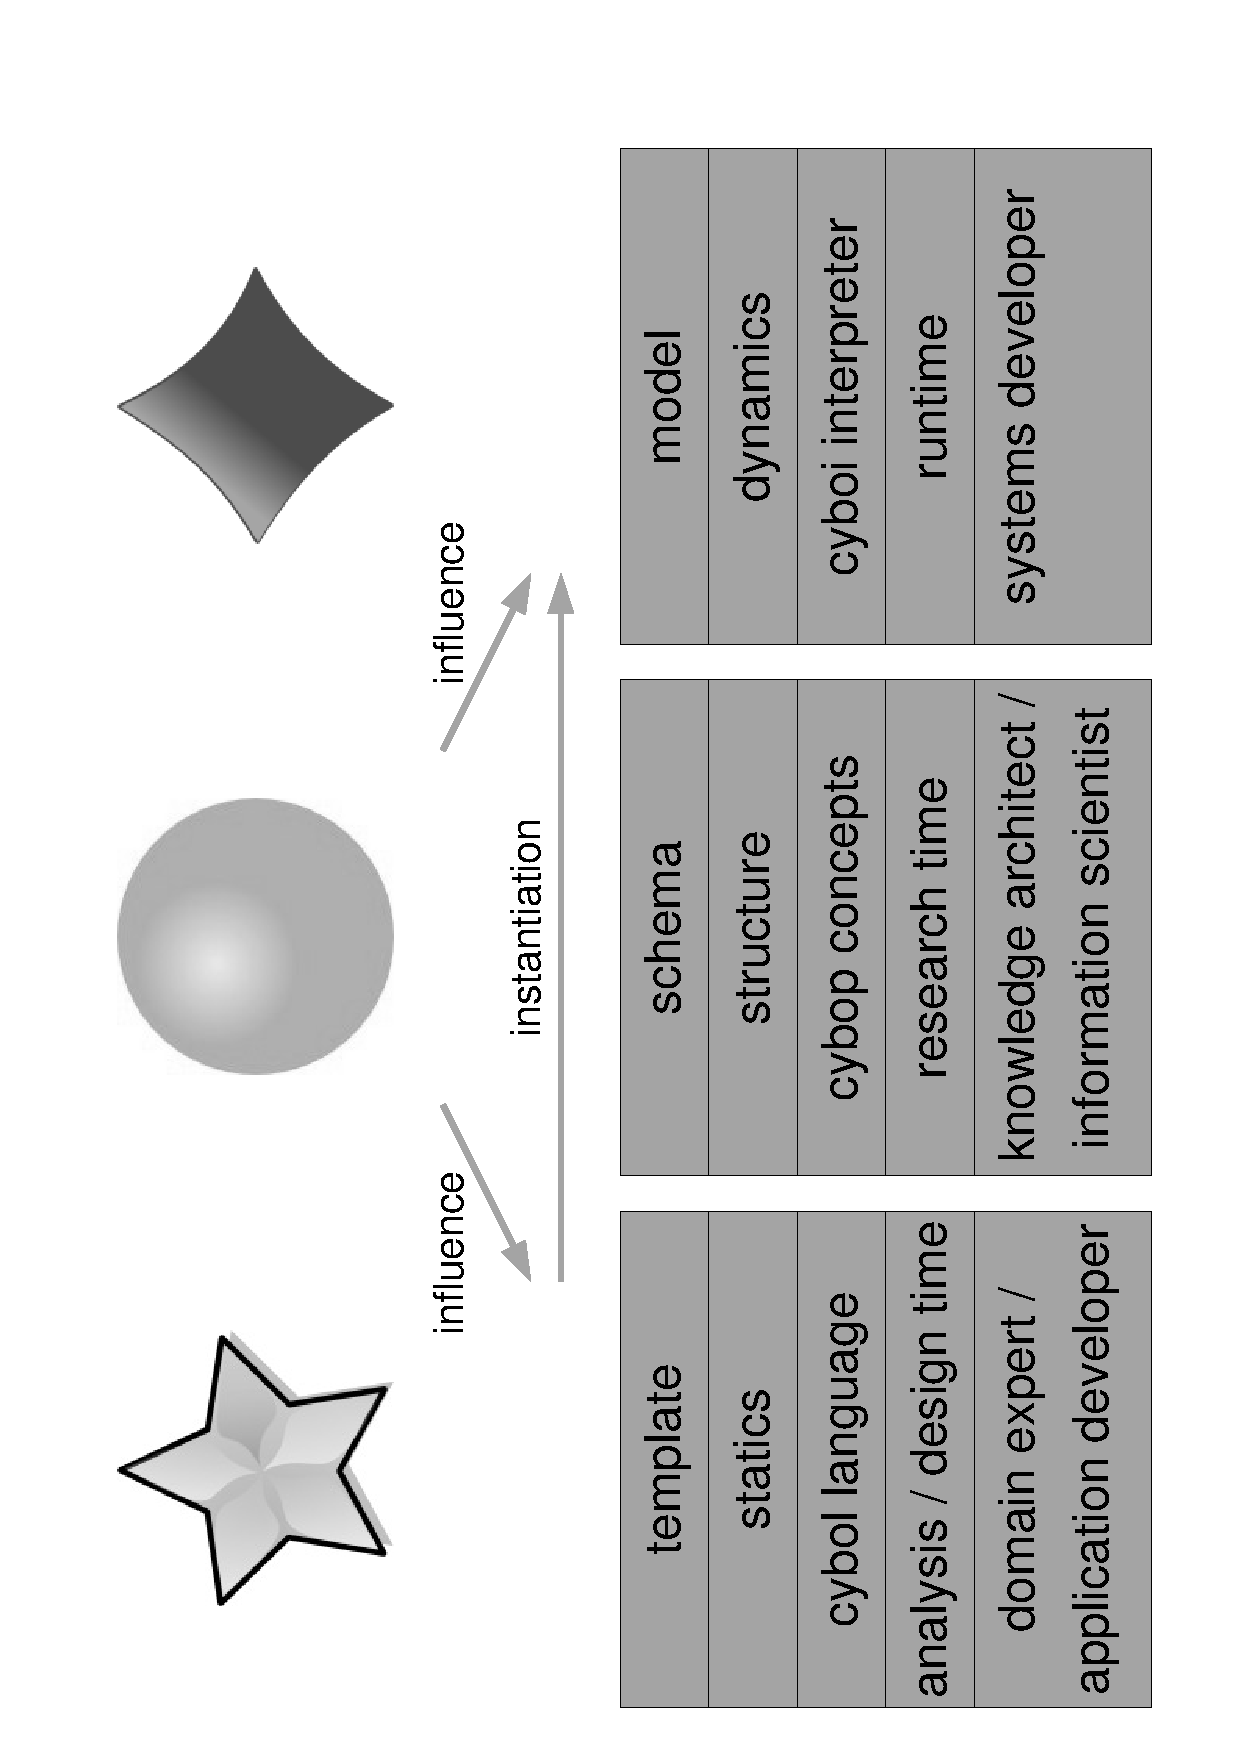
\includegraphics[scale=0.3,angle=-90]{graphic/triumvirate.pdf}
        \caption{Knowledge Triumvirate with Schema, Template and Model}
        \label{triumvirate_figure}
    \end{center}
\end{figure}

All three of them are closely connected (figure \ref{triumvirate_figure}): The
CYBOP knowledge \emph{Schema} provides a structure for both, knowledge
templates and -models; CYBOI \emph{Models} are the dynamic runtime instances of
static design-time CYBOL \emph{Templates}.

One reason for the mix-up of domain knowledge and system control in traditional
applications is the lack of a comprising solution for knowledge representation.
Software systems always have to fall back to using programming paradigms that
introduce more and more dependencies, as the system grows. John F. Sowa
\cite{sowa} writes:

\begin{quote}
    The enhanced productivity of the \emph{Fourth Generation Languages} (4GL),
    the \emph{Object Oriented Programming Systems} (OOPS) and the
    \emph{Computer Aided Software Engineering} (CASE) tools is derived from a
    common strength: improved methods of representing application knowledge in
    a form that can be used and reused by multiple system components. Their
    limitations result from a common weakness: the inability to share that
    knowledge with systems that use a different representation. The potential
    for conflict is inevitable: sharing requires a common representation, but
    independently developed systems almost invariably use different
    representations. In order to support knowledge sharing among heterogeneous
    systems, the conceptual schema must be general enough to accommodate anything
    that can be represented in any current system, any legacy system inherited
    from the past, and any new system that may be developed in the future.
\end{quote}

CYBOP claims to provide just that -- a common schema for knowledge
representation and -exchange. If not perfect, it is certainly a first step
towards an all-general knowledge schema.

Section \ref{functional_programming_heading} contained a quote in which the
\emph{Association of Lisp Users} \cite{commonlisp} states that, other than
\emph{Functional Programming}, \emph{Procedural Languages} essentially performed
everything as \emph{Side Effects} (variable updates persisting after expression
evaluation) to data structures. \textit{A purely procedural language}, after
\cite{commonlisp}, \textit{would have no functions, but might have subroutines
of no arguments that returned no values, and performed certain assignments and
other operations based on the data it found stored in the system.} This is
almost how CYBOI manipulates its knowledge -- in the manner of one huge side
effect. Its procedures do forward some parameters, but only one of these is
really application-related: the \emph{Knowledge Tree}. State- and logic
knowledge given in form of CYBOL templates are not bundled with low-level CYBOI
procedures. Both are configurable knowledge. Logic knowledge models do not get
input/ output (i/o) parameters handed over directly, but as dot-separated path
to the corresponding value in the knowledge tree.

Because all knowledge is stored in tree-form, application systems become much
more flexible than complex class networks as known from object-oriented
programming. Tree structures are easy to edit, with or without supportive tools.
They allow to better estimate necessary changes caused by new requirements,
because dependencies are obvious. Software maintenance gets improved, because
application developers can focus on pure domain knowledge; low-level system
functionality is provided by CYBOI. CYBOL applications are therefore absolutely
portable between platforms, as long as these were already considered in the
underlying CYBOI. Due to the straight-forward possibility of accessing parts of
a knowledge tree along well-defined paths, applications may win in performance.

%%
% $RCSfile: philosophical_parallels.tex,v $
%
% Copyright (C) 2002-2008. Christian Heller.
%
% Permission is granted to copy, distribute and/or modify this document
% under the terms of the GNU Free Documentation License, Version 1.1 or
% any later version published by the Free Software Foundation; with no
% Invariant Sections, with no Front-Cover Texts and with no Back-Cover
% Texts. A copy of the license is included in the section entitled
% "GNU Free Documentation License".
%
% http://www.cybop.net
% - Cybernetics Oriented Programming -
%
% http://www.resmedicinae.org
% - Information in Medicine -
%
% Version: $Revision: 1.1 $ $Date: 2008-08-19 20:41:08 $ $Author: christian $
% Authors: Christian Heller <christian.heller@tuxtax.de>
%

\subsection{Philosophical Parallels}
\label{philosophical_parallels_heading}

- Tree of Porphyry (p. 5) and Brentano's category tree (\cite{sowa} p. 57)
- How are Plato's / Aristotle's basic categories weaved into CYBOP model?
  - quality + quantity in part\_model
  - activity = cyboi; passivity = cybol
  - having + situated = compound (has parts; a part is part of (= situated in) a whole)
  - spatial + temporal (+ mass) = meta knowledge about parts

%
% $RCSfile: common_knowledge_abstraction.tex,v $
%
% Copyright (C) 2002-2008. Christian Heller.
%
% Permission is granted to copy, distribute and/or modify this document
% under the terms of the GNU Free Documentation License, Version 1.1 or
% any later version published by the Free Software Foundation; with no
% Invariant Sections, with no Front-Cover Texts and with no Back-Cover
% Texts. A copy of the license is included in the section entitled
% "GNU Free Documentation License".
%
% http://www.cybop.net
% - Cybernetics Oriented Programming -
%
% http://www.resmedicinae.org
% - Information in Medicine -
%
% Version: $Revision: 1.1 $ $Date: 2008-08-19 20:41:05 $ $Author: christian $
% Authors: Christian Heller <christian.heller@tuxtax.de>
%

\subsection{Common Knowledge Abstraction}
\label{common_knowledge_abstraction_heading}
\index{Common Knowledge Abstraction}
\index{Software Engineering Process}
\index{SEP}
\index{Analysis}
\index{Design}
\index{Implementation}
\index{Abstraction Gaps}
\index{CYBOL}
\index{CYBOI}

Although this work does not address the \emph{Software Engineering Process}
(SEP) directly, its results have great effect on it, which this section wants to
shed some more light on. Classical SEP phases are: \emph{Analysis}, \emph{Design}
and \emph{Implementation} (chapter \ref{software_engineering_process_heading}).

\begin{figure}[ht]
    \begin{center}
        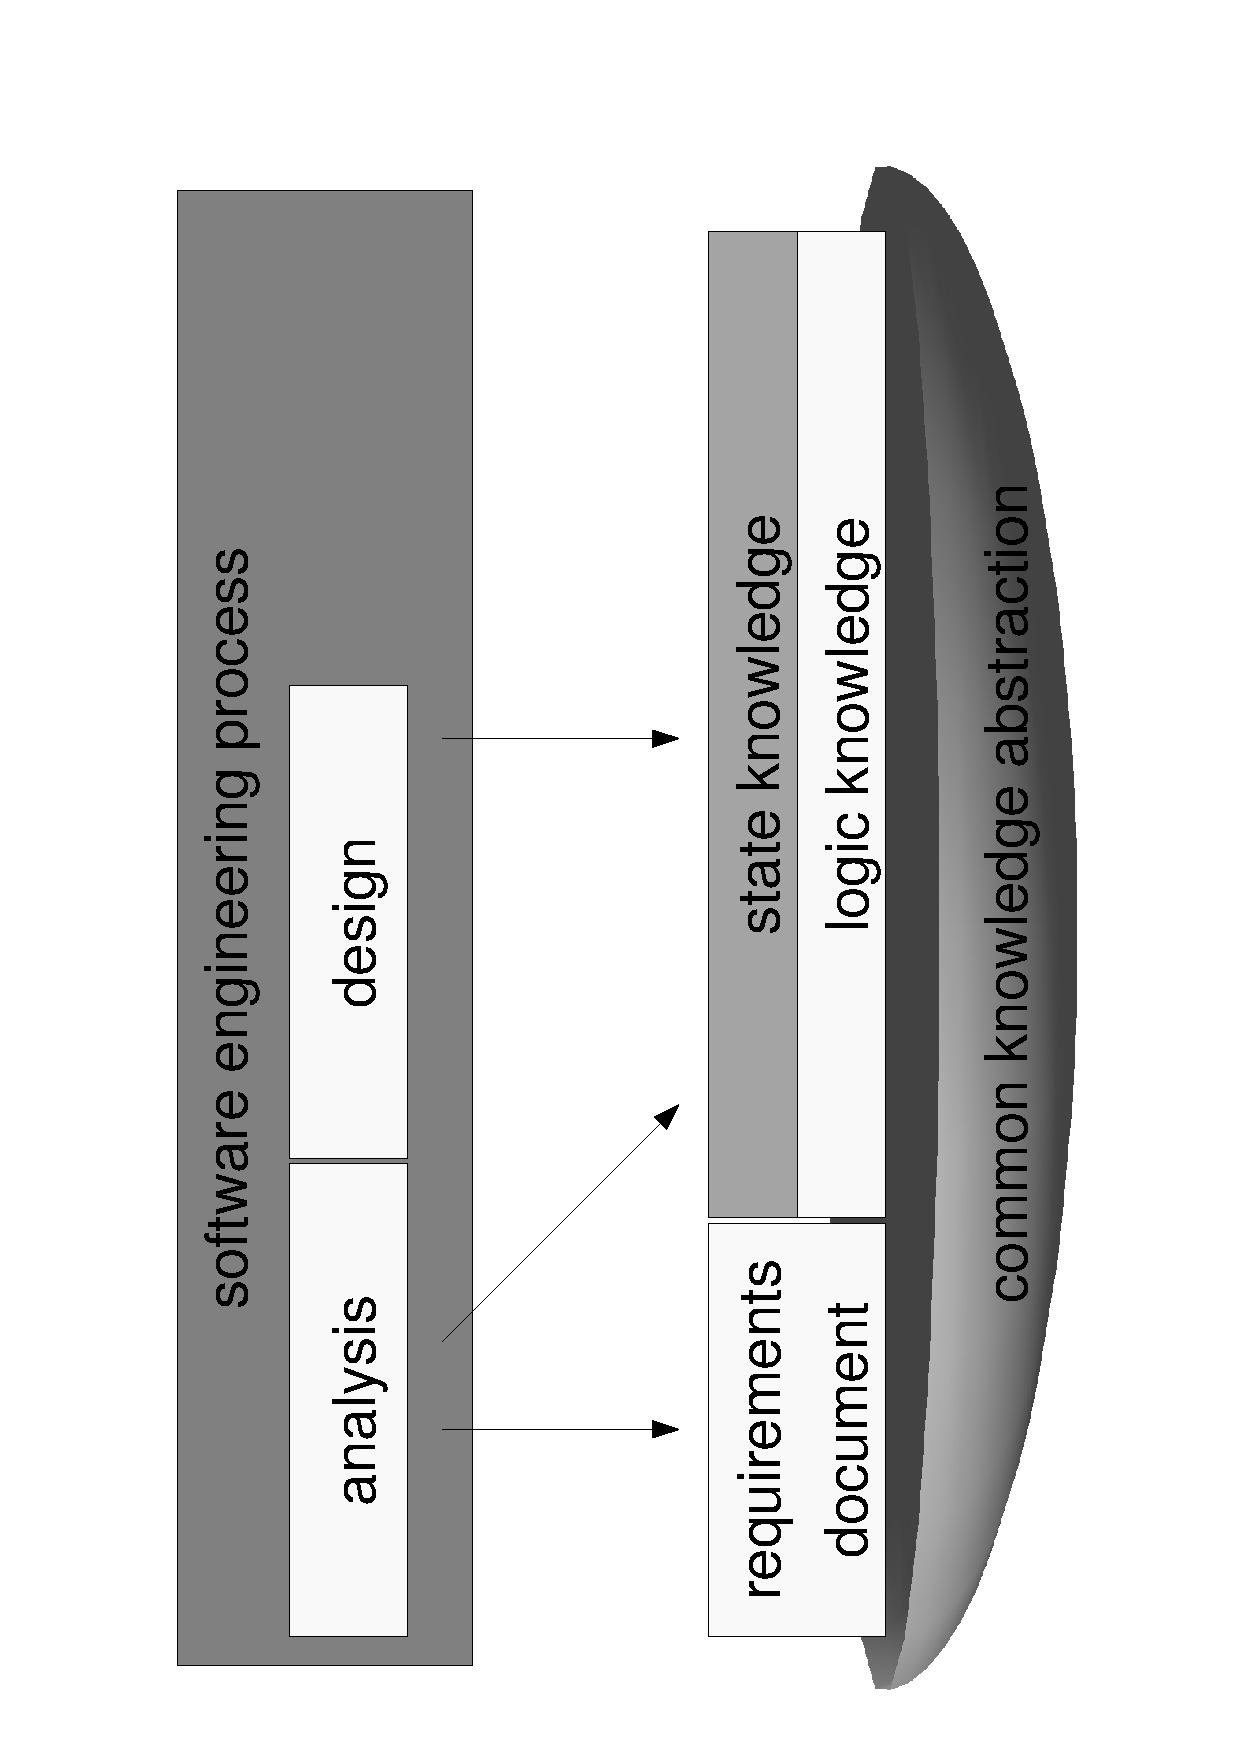
\includegraphics[scale=0.3,angle=-90]{graphic/common.pdf}
        \caption{Common Knowledge Abstraction useable by many SEP Phases}
        \label{common_figure}
    \end{center}
\end{figure}

Section \ref{abstraction_gaps_heading} pointed out abstraction gaps and
multiple development paradigm switches, happening during a software project's
lifetime. It set out to find a \emph{Common Knowledge Abstraction} for all
phases. The results of this work overcome \emph{Gap 2}, as shown in figure
\ref{gaps_figure}. Knowledge models as specified in this work can be used
throughout most project phases (figure \ref{common_figure}). Domain experts and
application developers work with platform-neutral knowledge templates. Since
these are interpreted, a translation into classical software source code is not
necessary anymore. CYBOL knowledge templates represent the designed
architecture \emph{and} implemented application, at the same time. The formerly
needed implementation phase thus disappears, which shortens the whole SEP. It
is hard to estimate the amount of saved time and costs.

Using CYBOL, experts can hopefully yet more actively contribute to application
development. Consequently, there may be less organisational problems in
projects and companies, if experts and system developers can independently
develop their parts (CYBOL vs. CYBOI) of the application system to be created.
The whole SEP may become more \emph{transparent} and \emph{understandable}, and
hopefully produce more \emph{flexible}, \emph{stable} and \emph{secure}
systems. However, the exact effort, especially to what concerns security issues
cannot be estimated yet and has to be investigated further.

%
% $RCSfile: long-life_software_system.tex,v $
%
% Copyright (C) 2002-2008. Christian Heller.
%
% Permission is granted to copy, distribute and/or modify this document
% under the terms of the GNU Free Documentation License, Version 1.1 or
% any later version published by the Free Software Foundation; with no
% Invariant Sections, with no Front-Cover Texts and with no Back-Cover
% Texts. A copy of the license is included in the section entitled
% "GNU Free Documentation License".
%
% http://www.cybop.net
% - Cybernetics Oriented Programming -
%
% http://www.resmedicinae.org
% - Information in Medicine -
%
% Version: $Revision: 1.1 $ $Date: 2008-08-19 20:41:07 $ $Author: christian $
% Authors: Christian Heller <christian.heller@tuxtax.de>
%

\subsection{Long-Life Software System}
\label{long-life_software_system_heading}
\index{CYBOP Long-Life Software System}
\index{CYBOI}
\index{CYBOL}
\index{SPP}
\index{OOP}
\index{CYBOP Knowledge Schema}
\index{Knowledge Template}
\index{Knowledge Model}

The pure existence of proper knowledge does not suffice to create an improved
kind of software system, within a slimmer software development process. The new
systems need to know how to \emph{handle} knowledge, at runtime. The criticism
is twofold, because traditionally:

\begin{enumerate}
    \item Operating systems do not have sufficient knowledge handling capabilities
    \item Applications contain too much low-level system control functionality
\end{enumerate}

This is changed when using CYBOP. The active CYBOI interpreter encapsulates
memory allocation, persistence- and communication mechanisms, signal handling,
logging facilities and more, which belong to the system level. While
traditional programming philosophies try to make these \emph{reusable}, CYBOI
implements them just once, in a manner that \emph{all} applications can access
and use them. As a side-effect, the need for the study and repeated application
of software patterns disappears. Additionally, and most importantly, CYBOI
knows how to handle knowledge provided in form of passive CYBOL templates.

Although still dependent on an underlying operating system (for hardware device
drivers and more), CYBOI is developing towards becoming one itself. Applications,
on the other hand, do not have to care about communication paradigms and other
low-level issues anymore; their focus is pure domain knowledge, encoded in CYBOL.

%CYBOI's \emph{Exokernel} OS architecture provides security.
%All signals have to pass one control loop which invokes signal handling routines.
%So they all can be checked.
%CYBOI's architecture is thus similar to \emph{Software Agent} systems.

In classical type-based systems, no matter whether created in an SPP- or OOP
language, the type of data needs to be known to find out about their structure
and functionality. In CYBOP systems, all compound knowledge models have the
same structure. Since they do not differ, they can be manipulated in the same
manner. Only types (the kind of abstraction) of state primitives and logic
operations need to be distinguished.

CYBOL knowledge templates, of which a \emph{Clone} is made when a knowledge
model (instance) gets created, are \emph{not} treated as types. Once a
knowledge model exists, its original knowledge template can never be accessed
by it again, since a model holds no reference to its template. A template
merely delivers the initial values for the model instantiated from it. After
creation, a model exists on its own. It can be used and modified independently
of any types, and is thus absolutely flexible.

But that also means that systems implementing the CYBOP knowledge schema are
more future-proof. Unforeseeable requirements can be implemented anytime,
without a static type model having to be changed, without fragile classes
having to be considered, without dependencies causing existing functionality to
break. CYBOP systems are therefore \emph{Long-Life Systems} without
architectural decay. Domain-/ application model changes do neither affect the
structure of the knowledge schema, nor other parts of the static architecture
of the underlying CYBOI interpreter.

The argument that systems developed in this manner were not safe because they
lacked the constraints defined by a type does not hold, since also classical
systems permit runtime objects to get manipulated, and to be assigned values
not matching their type. In this case, of course, the system is alerted with an
error, but in the end it is always the application developer who has to handle
-- or better prevent such errors.


%
% $RCSfile: limits.tex,v $
%
% Copyright (C) 2002-2008. Christian Heller.
%
% Permission is granted to copy, distribute and/or modify this document
% under the terms of the GNU Free Documentation License, Version 1.1 or
% any later version published by the Free Software Foundation; with no
% Invariant Sections, with no Front-Cover Texts and with no Back-Cover
% Texts. A copy of the license is included in the section entitled
% "GNU Free Documentation License".
%
% http://www.cybop.net
% - Cybernetics Oriented Programming -
%
% http://www.resmedicinae.org
% - Information in Medicine -
%
% Version: $Revision: 1.1 $ $Date: 2008-08-19 20:41:07 $ $Author: christian $
% Authors: Christian Heller <christian.heller@tuxtax.de>
%

\section{Limits}
\label{limits_heading}
\index{CYBOP Limits}

Naturally, there are \emph{Limits} to CYBOP. For instance, it:

\begin{itemize}
    \item[-] does not claim to be \emph{the} approach for all kinds of
        programming problems, although it thinks to contribute suitable
        concepts for at least standard business application development.
        However, its usability for hardware-close systems with Real Time (RT)
        requirements, or for control engineering is questionnable and yet to be
        investigated;
    \item[-] depends on the existence of a system with knowledge-processing
        capabilities, which current \emph{Operating Systems} (OS) are not. The
        CYBOI delivered with it is quite mature, but still lacks functionality
        like different \emph{User Interfaces} (UI), various \emph{import/ export}
        (i/e) filters/ translators, better error handling, prioritising and
        further OS features. Only functionality already implemented in CYBOI can
        also be used in CYBOL. But because CYBOI is free software, continuously
        developed in an open project, new features shall be implementable shortly;
    \item[-] has no type-checking features like classical compilers. This is
        the cost of flexibility. The knowledge schema is the only type
        structure provided by CYBOI. All domain- and application knowledge is
        hold externally, in CYBOL knowledge templates, and interpreted only at
        runtime;
    \item[-] will have performance problems when using UI models, especially
        graphical ones, because these are sent in complete to the graphics
        adapter card, whenever a minor change is made. Techniques have to be
        found, that update only clips of a UI model, in graphics memory. The
        difficulty herein is that CYBOL application knowledge has \emph{no}
        direct access to system-level functionality;
    \item[-] does not eliminate all abstraction gaps in a SEP. Requirements
        described informally by an analysis document have to be mapped to CYBOL
        knowledge templates, which then represent the application to be created.
        Although analysts and experts may create CYBOL models right from the
        project start, there will probably never be a true replacement for the
        written requirements analysis document, as one form of abstraction.
        However, if not the informal descriptions of its models, the document
        itself may be created in CYBOL, since it represents knowledge.
\end{itemize}

%\input{persistency}
%Ein Haupt-Denkproblem habe ich immer noch mit persistent gemachten
%Laufzeit-Modellen. Z.B. koennte man in einer Personalverwaltung die
%personenbezogenen Daten in einer CYBOL Datei speichern und die
%Adressdaten in einer anderen CYBOL Datei, aehnlich, wie man Datensaetze
%in verschiedenen Tabellen einer relationalen DB ablegt. Jede CYBOL Datei
%wuerde als Namen eine eindeutige ID bekommen und im Datensatz einer
%Person wuerde als Adressfeld lediglich die ID der Adresse als Verweis
%stehen. Doch wie sage ich einem System, welche Daten es zusammen, und
%welche in getrennten Dateien speichern soll?

